% Created 2013-07-29 Mon 20:04
\documentclass[a4paper,11pt]{article}
\usepackage[utf8]{inputenc}
\usepackage[T1]{fontenc}
\usepackage{hyperref}
\tolerance=1000
\usepackage{fontspec}
\usepackage{biblatex}
\usepackage{graphicx}
\usepackage{fullpage}
\usepackage{caption}
\usepackage{subfig}
\usepackage{hyperref}
\usepackage{moreverb}
\usepackage{fancyvrb}
\usepackage[ruled]{algorithm2e}

\bibliography{report}
\defaultfontfeatures{Mapping=tex-text}
\setromanfont[Ligatures={Common},Numbers={Lining}]{Linux Libertine}
%\setmonofont{Liberation Mono}   

\newsavebox{\boxone}
\newsavebox{\boxtwo}
\newsavebox{\boxthree}
\newsavebox{\boxfour}

\title{Sokoban: Search in a complex domain}
\author{Yann Chazzalon,  Nicolas Dossou-Gb{\'e}t{\'e}, Tony Chan Ki Hong and Michal Staniaszek}
\date{\today}

\begin{document}

\maketitle

\begin{abstract}
  a brief summary of your project and obtained results
\end{abstract}

\begin{figure}[!ht]
  \captionsetup[subfigure]{labelformat=empty}
  \centering
  \subfloat[\centering Yann Chazallon\\ 91/01/16]{
    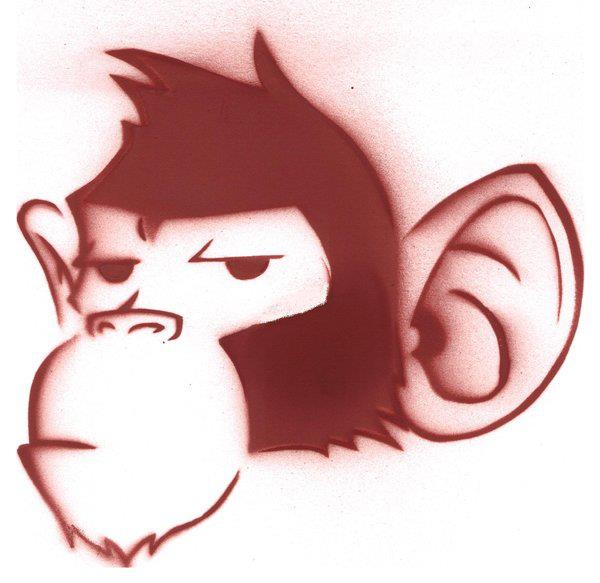
\includegraphics[width=.2\textwidth]{img/yann.jpg}
  }\quad
  \subfloat[\centering Nicolas Dossou-Gb{\'e}t{\'e}\\ 89/09/26]{
    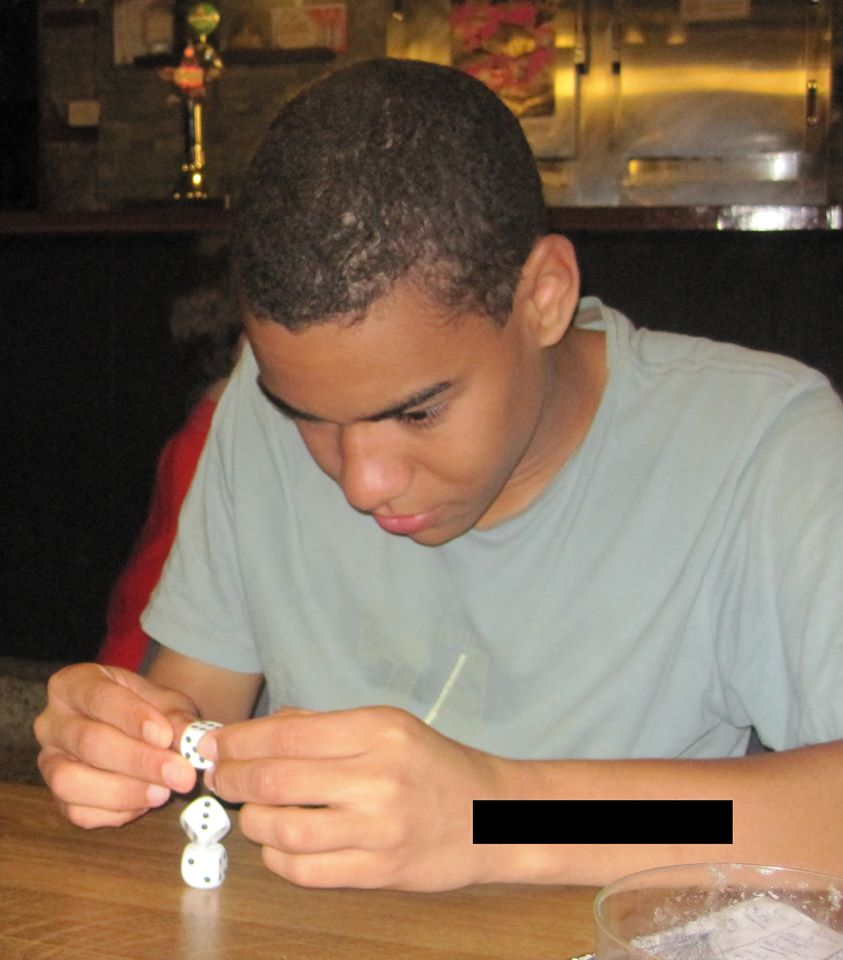
\includegraphics[width=.2\textwidth]{img/nicolas.jpg}
  }\quad
  \subfloat[\centering Tony Chan Ki Hong\\ /07/25]{
    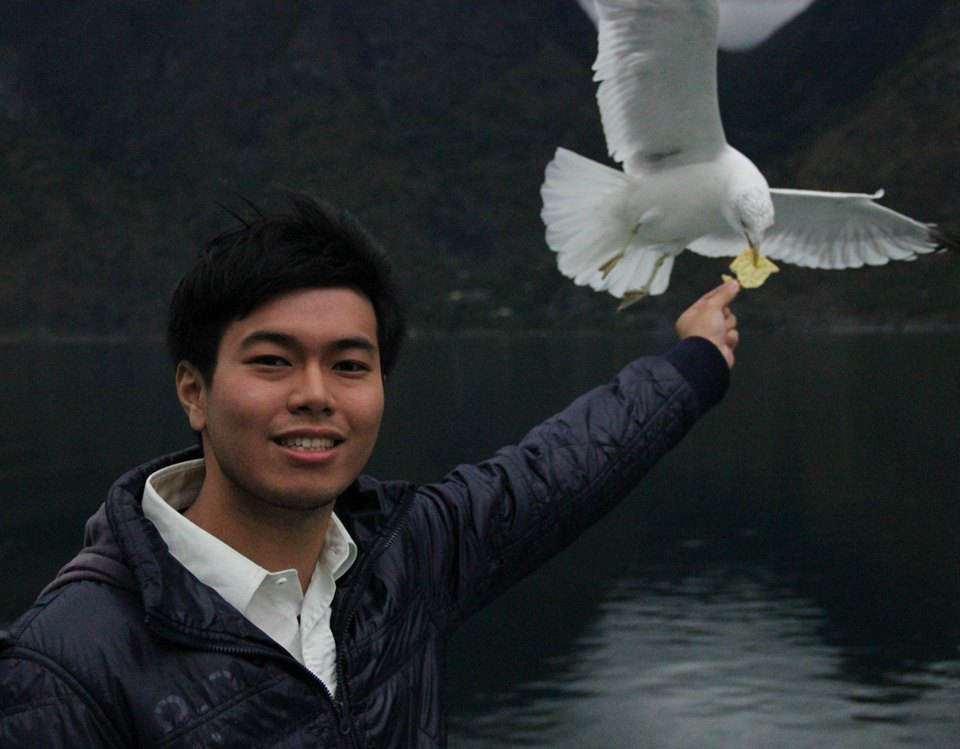
\includegraphics[width=.2\textwidth]{img/tony.jpg}
  }\quad
  \subfloat[\centering Michal Staniaszek\\ 90/12/07]{
    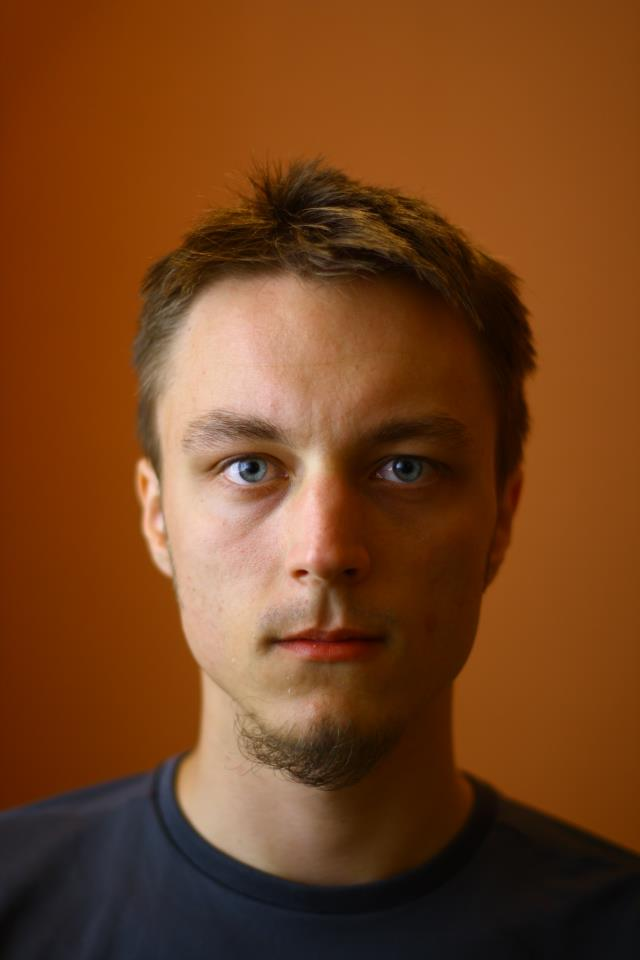
\includegraphics[width=.2\textwidth]{img/michal.jpg}
  }
\end{figure}

\section{Introduction}
\emph{Sokoban} is a puzzle game which written in 1981 by Hiroyuki Imabayashi. First published in 1982, it is now a very popular game, with many clones available on the internet. The player controls a warehouse keeper (for which \emph{sokoban} is the Japanese word), whose job it is to push boxes onto goal locations on the map. The player can move in four directions (up, down, left or right) on the map, which is split into discrete cells. The player can push boxes, but is unable to pull them. To be able to push a box, the player must be adjacent to it, and there must be an empty space behind the box into which it can be pushed. Only one box can be moved at a time; if two boxes are contacting each other, pushing one box does not move the other. While there are many graphical implementations, there are also many text-based implementations which use symbols for representing parts of the board, an example of which is shown in Figure \ref{fig:mapex}.

\begin{lrbox}{\boxone}
  \begin{minipage}{.25\textwidth}
\centering
\begin{BVerbatim}
#######
#  .@ #
# #.# #
#   $ #
#.$$ ##
#  ###
####
\end{BVerbatim}
  \end{minipage}
\end{lrbox}%

\begin{lrbox}{\boxtwo}
  \begin{minipage}{.25\textwidth}
\centering
\begin{BVerbatim}
#######
#  .@ #
# #.# #
# $$  #
#*   ##
#  ###
####
\end{BVerbatim}
  \end{minipage}
\end{lrbox}%

\begin{lrbox}{\boxthree}
  \begin{minipage}{.25\textwidth}
\centering
\begin{BVerbatim}
#######
#  .@ #
# #.# #
#$ $  #
#*   ##
#  ###
####
\end{BVerbatim}
  \end{minipage}
\end{lrbox}%

\begin{lrbox}{\boxfour}
  \begin{minipage}{.25\textwidth}
\centering
\begin{BVerbatim}
#######
#  *  #
# #*# #
#  @  #
#*   ##
#  ###
####
\end{BVerbatim}
  \end{minipage}
\end{lrbox}%

\begin{figure}
  \subfloat[A basic map]{\usebox{\boxone}}
  \subfloat[Half solved]{\usebox{\boxtwo}}
  \subfloat[In an unsolvable state]{\usebox{\boxthree}}
  \subfloat[The solved map]{\usebox{\boxfour}}
  \caption{A typical \emph{Sokoban} map. The player is represented by \texttt{@}, or \texttt{+} when on a goal, boxes by \texttt{\$} or \texttt{*} on a goal, walls by \texttt{\#}, goals by a period, and empty space by a blank. The map in (c) is unsolvable, as the two boxes on the left are both against a wall. This is called a \emph{deadlock}.}
  \label{fig:mapex}
\end{figure}

The game has garnered some interest in the artificial intelligence (AI) community due to the difficulty of finding automatic solutions. Games are an ideal platform for the development and testing of AI techniques, as game environments are much simpler and less (or not at all) noisy, and also have sets of simple rules for interaction with the world. Working in such environments allows for more control and closer investigation of the relevant parts of the problem that is being considered. \emph{Sokoban} in particular is an interesting problem due to its high branching factor, and the depth of the search trees that are generated when attempting to solve a problem. Even relatively simple problems can take upwards of 100 moves to solve, and more complex problems can exceed 500 moves, even in the optimal case. Additionally, it is possible to extend the search tree indefinitely---there is no time limit, and boxes can be pushed without restraint, so long as the push is valid. The branching factor is the total number of valid actions that can be applied to any box reachable from the player's current position. In the worst case, if there are $N$ boxes, all of which are accessible and can be pushed in any direction, the factor is $4N$ (each box can be pushed in 4 directions). Although in practice it is not possible to access all boxes, or push them in an arbitrary direction, but most maps have a large enough number of boxes that the branching factor has a large impact on the number of states expanded.

\section{Method}
\subsection{Map Representation}
\subsection{Deadlock Detection}
a description of your approach to the problem and your method
\section{Implementation}
\begin{algorithm}
  \DontPrintSemicolon
  \KwData{Search implementations forwards and backwards, initialised with start and goal.}
  \KwResult{A list of tuples of (\texttt{point}, \texttt{int}) containing motion of boxes from start to goal.}

  \Begin{
    current $\longleftarrow$ forwards\;
    opposite $\longleftarrow$ backwards\;
    new $\longleftarrow \emptyset$\;
    key $\longleftarrow $ \texttt{null}\;
    \Repeat{key $\neq$ \texttt{null}}{
      swap current and opposite\;
      new $\longleftarrow$ current.step()\;
      \lIf{node $\in$ new $\land$ node $\in$ opposite.open}{key $\longleftarrow$ node}
    }
    fkey $\longleftarrow$ forwards.open.get(key)\;
    bkey $\longleftarrow$ backwards.open.get(key)\;
    fActions $\longleftarrow$ fkey.unwind()\;
    bActions $\longleftarrow$ bkey.unwind()\;
    \Return merge(fActions, bActions.reverse())\;
  }
\caption{Bi-directional search}
\end{algorithm}

implementation details (if there are any important ones)
\section{Evaluation}
experimental evaluation and a thorough analysis of your results. This section should include:
How well did your agent do on the different maps?
\section{Discussion}
reflection section dealing with questions: How did you plan to solve the problem? How did you plan the work in the group? What other methods did you try out? What did work/ did not work? Why? How did you end up with the current approach? How did you measure the performance and success during the process? How would you solve it if you were asked to do it again given what you know now?

\printbibliography

\end{document}